\section{Exploratory Thinking in Children through Patterning}
Children are extraordinary explorers. Unprohibited by set structures and knowledge of available representations \cite{hinds2001,tversky1973availability,wiley1998expertise}, children can come up with more unusual hypotheses and explanations than adults \cite{gopnik2017,lucas2014children,wilson2021}. Interestingly, where adults tend to fixate and satisfice \cite{jansson1991design, kershaw2004, Ohlsson1992, simon1972theories}, children demonstrate cognitive flexibility and even a bias towards exploration \cite{gopnik2017,lucas2014children,sumner2019exploration,sumner2019}. Given children’s propensity for exploration, how might exploration be used as a pedagogical tool? Compared to direct instruction or worked examples, exploration strategies can support better engagement and discovery learning, leading to improved transfer of knowledge to new problems \cite{bonawitz2011double,Glogger-Frey2015,Schwartz2004}. However, pure exploration and unguided learning can be inefficient and induce a heavy cognitive load \cite{kirschner2006,tuovinen1999comparison}. We hypothesize that for the domain of pattern learning, directed exploration will yield more productive results \cite{Kapur2008,wilson2021}. 

We investigate exploration as a learning strategy compared to a demonstration of a pattern for preschool and kindergarten-aged children. Patterning is an important skill for children, particularly in learning algebraic mathematics \cite{papic2011assessing}. Young children may gravitate toward patterning activities because no alphanumeric knowledge is needed to engage in them. Prior studies show that children as young as four years old can recognize and abstract (create the same pattern using new materials) repeating pattern units \cite{fyfe2015,rittle2013}. Though patterning interventions improve children's mastery of specific patterns, they still often struggle to transfer their knowledge to new contexts, especially when assessed on their ability to recognize the unit of repeat \cite{fyfe2015,papic2007growth}. Given the success of exploratory learning strategies on knowledge transfer in other domains of learning \cite{bonawitz2011double,Glogger-Frey2015,Schwartz2004}, we compare whether exploration will facilitate implicit pattern recognition and transfer of patterning ability more than a demonstrated example of the pattern.

\subsection{Experiment: Can Exploration Improve Pattern Learning?}

\subsubsection{Participants}
We recruited participants via emails collected from an online research database. 68 children, aged five to six years old (mean age$=5.98$, $SD=0.58$) participated in this study. Of these children, 34 were five-year-olds, and 34 were six-year-olds (10 children were excluded from analyses due to failing pretest items or technical difficulties that prevented completion of the study). Children were split into either the \textit{exploration} or \textit{demonstration} conditions. In the \textit{exploration} condition, participants engaged with the pattern materials directly while \textit{demonstration} condition participants watched the experimenter engage with the pattern materials. The experiment design was yoked, meaning that for each participant in the \textit{exploration} condition, a paired participant in the \textit{demonstration} condition would see the same information in the same order as the participant in the \textit{exploration} condition. All pairs of participants were age-matched.

\subsubsection{Procedure}
The experiment took place over the videoconferencing platform Zoom with a prototype developed in Google Slides to allow for synchronous observation and communication between the child participant and experimenter. Parents were instructed to not interfere with the child's performance unless in the case of technical difficulty. The patterns within the prototype consisted of various shapes created with the Shapes tool in Google Slides. Children interacted with the shapes by clicking and dragging them, with help from the experimenter or parent if needed. After a pattern duplication task, the experiment consisted of a pattern abstraction pre-test and a pattern learning task. A pattern transfer and pattern abstraction post-task followed pattern learning. After the full experiment, children and parents were debriefed and received a \$5 USD gift card for their time and participation in the 10-15 minute experiment. Pattern duplication and abstraction tasks were adapted from \cite{rittle-johnson2007}; pattern learning and transfer tasks were novel tasks designed for this study.

\subsubsection{Tasks}

\textit{Pattern Duplication Task.} Participants saw a model two-unit AAB pattern and were asked to duplicate the pattern using materials of the same shape and color. The pattern was considered correct if at least one unit of the solve pattern matched the model pattern. This task served as exclusionary criteria for the study. 

\textit{Pattern Abstraction Pre- \& Post-Tests.} The abstraction pre- and post-tests consisted of a two-unit ABB model pattern and a two-unit AAB model pattern. The experimenter asked children to create the same pattern using materials of different shapes and colors than the model pattern. The pattern was considered correct if at least one unit of the solve pattern matched the model pattern. Children completed the abstraction tasks both before and after the pattern learning and transfer tasks as a measure of learning or improvement.

\begin{figure}
\centering
  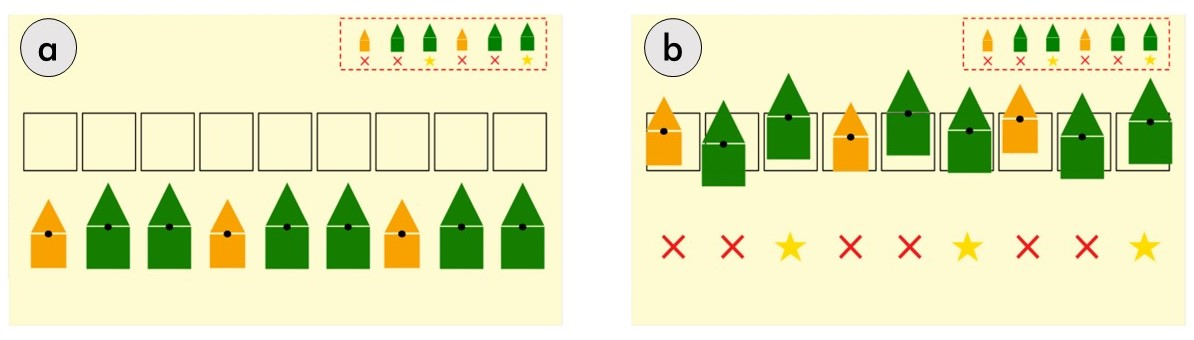
\includegraphics[width=0.9\textwidth]{future/figures/pattern_learn.jpg}
  \caption[The pattern learning task consists of three units of an ABB pattern with house shapes and a small icon to remind children of the underlying pattern.]{a) The pattern learning task consists of three units of an ABB pattern with house shapes and a small icon to remind children of the underlying pattern. b) Children can reveal the contents of the houses to to find the hidden stars underneath. \textit{Exploration} condition children chose the order in which the houses were revealed while \textit{demonstration} condition children watched the experimenter reveal the houses in the order of their age-matched \textit{exploration} counterpart.
}
  \label{fig:pattern-learn}
\end{figure}

\textit{Pattern Learning Task.} The pattern learning task consisted of a row of nine house shapes of two sizes and colors: the orange houses were small shapes, and the green houses were big shapes. The nine houses formed a three-unit ABB pattern (small, large, large) (Figure \ref{fig:pattern-learn}a). The second `B’ shape in each ABB unit contained a star shape hidden underneath with all other house shapes hiding an 'x' underneath (Figure \ref{fig:pattern-learn}b). We informed all participants that their goal was to find the three stars by figuring out the pattern to find them. Participants in the \textit{exploration} chose the order in which to reveal the hidden contents of the nine house shapes. For the \textit{demonstration} condition participants, the experimenter moved all shapes for the participant in the same order as the participant’s paired \textit{exploration} condition counterpart. 

\textit{Pattern Transfer Task.} The pattern transfer task consisted of the same ABB pattern row as the pattern learning task, but with different shapes of different colors (red and purple lightbulbs)(Figure \ref{fig:pattern-transfer}a). As with the learning pattern, stars were hidden under the second B shape in each ABB unit (Figure \ref{fig:pattern-transfer}b). The experimenter explained that the participant could find the stars in the same place using the same pattern as the pattern learning task. A small thumbnail in the corner of the slide served as a reminder of the previous pattern from the learning task. The experimenter gave children five chances to try to find the three hidden stars, giving verbal feedback after each attempt. All children were told to choose five shapes even if they found all three stars prior to the fifth attempt.

\begin{figure}
\centering
  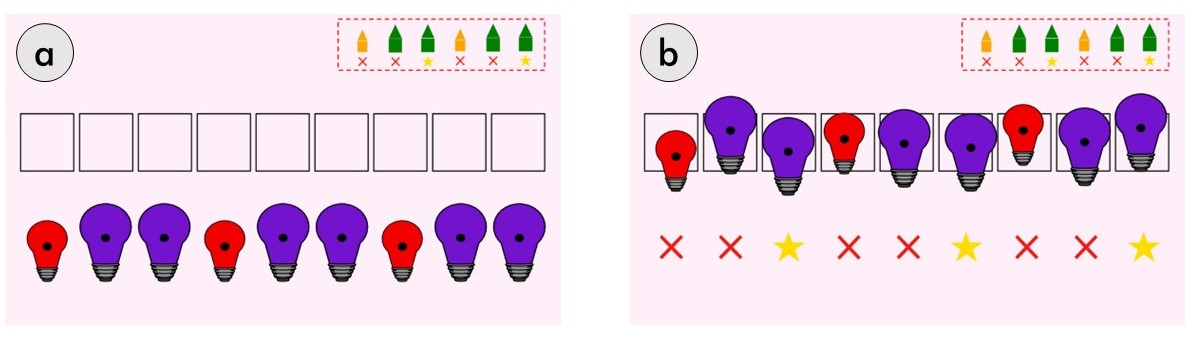
\includegraphics[width=0.9\textwidth]{future/figures/pattern_transfer.jpg}
  \caption[The pattern transfer task consisted of the same three-unit ABB pattern as the pattern learning task.]{a) The pattern transfer task consisted of the same three-unit ABB pattern as the pattern learning task with different shapes. b) Children had five chances to reveal any of the shapes to find the three hidden stars. A small icon in the corner reminded children of the pattern from the pattern learning task.
}
  \label{fig:pattern-transfer}
\end{figure}

\subsection{Preliminary Results}

\begin{figure}
\centering
  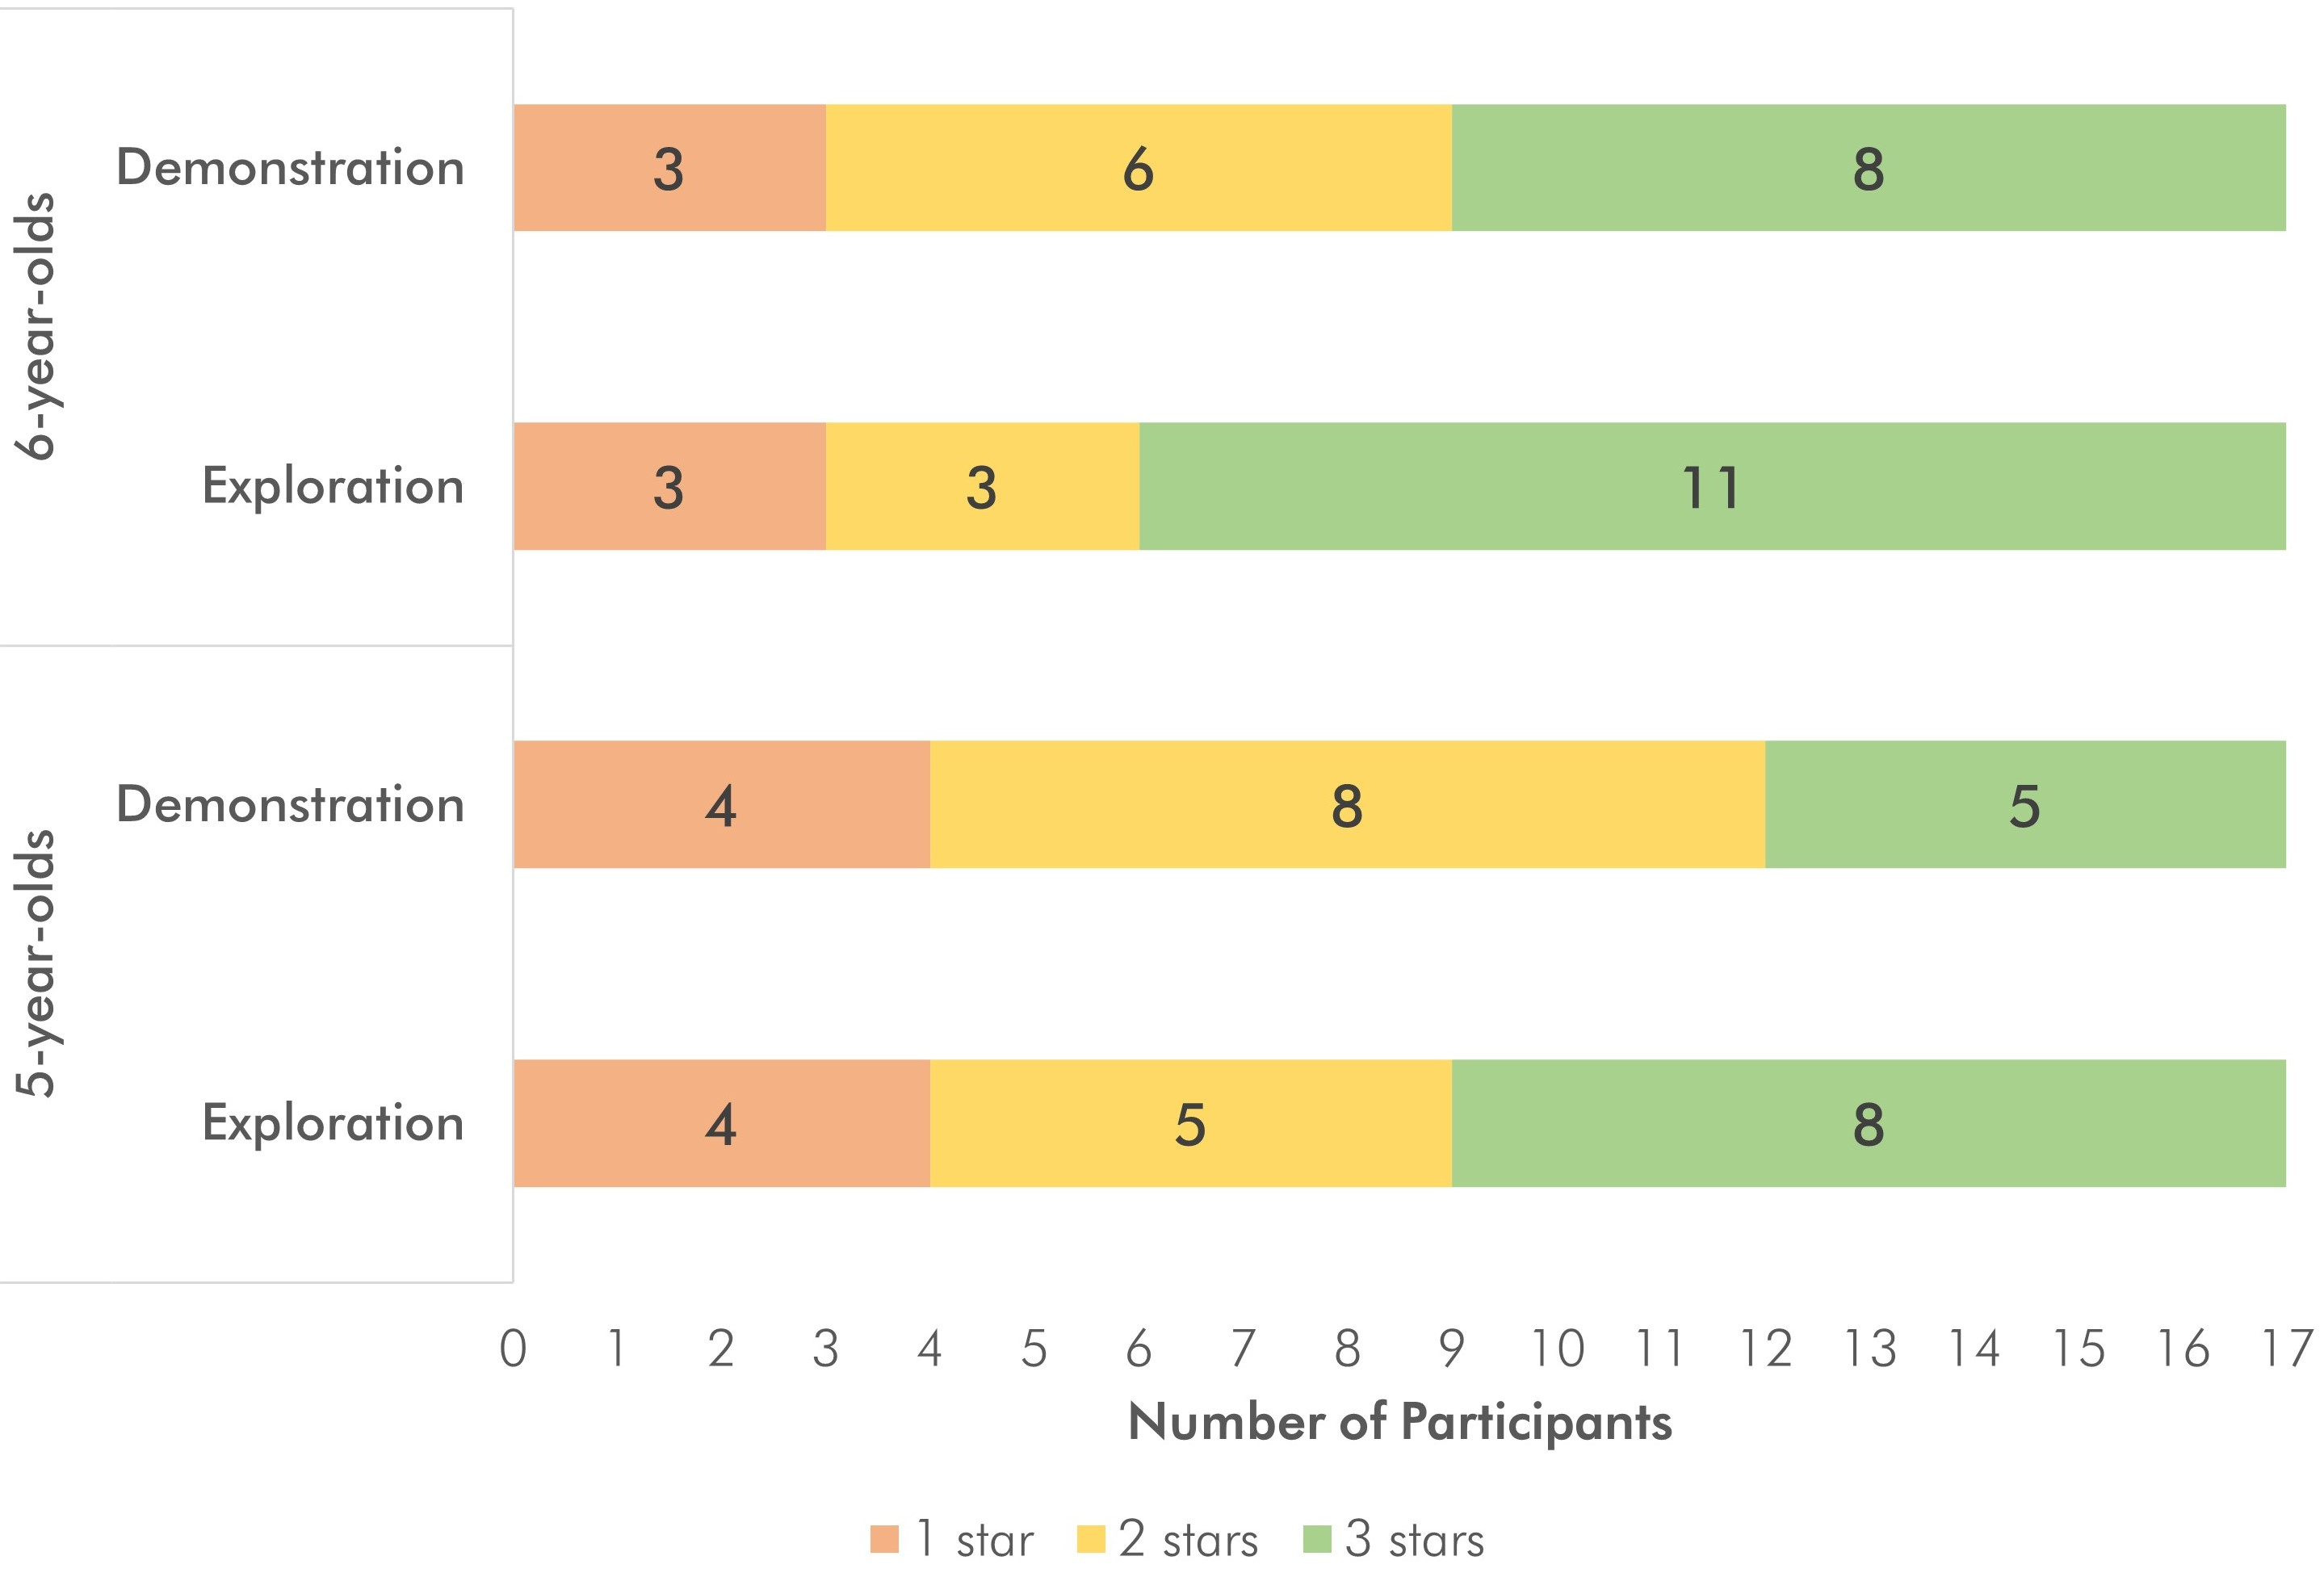
\includegraphics[width=.8\textwidth]{future/figures/pattern_stars.jpg}
  \caption{The number children who found one, two, and three hidden stars in the pattern transfer task ($n=17$ for each age group in both conditions; $n=34$ total in each condition). In both conditions, more six-year-olds successfully found all three stars compared to five-year-olds.
}
  \label{fig:pattern-stars}
\end{figure}

\subsubsection{No significant difference in pattern abstraction}
Pre- and post-test tasks were scored as a binary outcome for whether the pattern was correct or incorrect. We combined the two pre-tests and the two post-test scores into one pre-test and one post-test score with a total out of two for each. Children in both conditions performed nearly at ceiling for both pre- and post-abstraction tasks (\textit{exploration} pre-test $mean=1.79$, $SD=0.54$; post-test $mean=1.82$, $SD=0.52$. \textit{demonstration} pre-test $mean=1.91$, $SD=0.29$; post-test $mean=1.94$, $SD=0.24$). A linear regression with age as a covariate shows that the average difference from pre- to post-test was not significantly different ($F(2,65)=1.76, R^2=0.05, p=.18$).

\subsubsection{Six-year-olds recognize patterns better than five-year-olds}
In general, six-year-olds performed better on the pattern transfer task, with a larger proportion finding all three stars, demonstrating an understanding of the unit of repeat in the ABB pattern. In the \textit{exploration} condition, 8 of the 17 five-year-olds found all three stars compared to 11 of the 17 six-year-olds. In the \textit{demonstration} condition, 5 of the 17 five-year-olds found all three stars compared to 8 of the 17 six-year-olds. All participants found at least one star in the task. Figure \ref{fig:pattern-stars} shows the number of participants who found one, two, and three stars by age and condition. Though there are no significant differences between conditions in the preliminary data ($\chi^2=2.76, df=2, p=.25$), we observed a slight trend towards better performance in the \textit{exploration} condition.

\subsubsection{Exploration affects pattern learning strategies}

\begin{figure}
\centering
  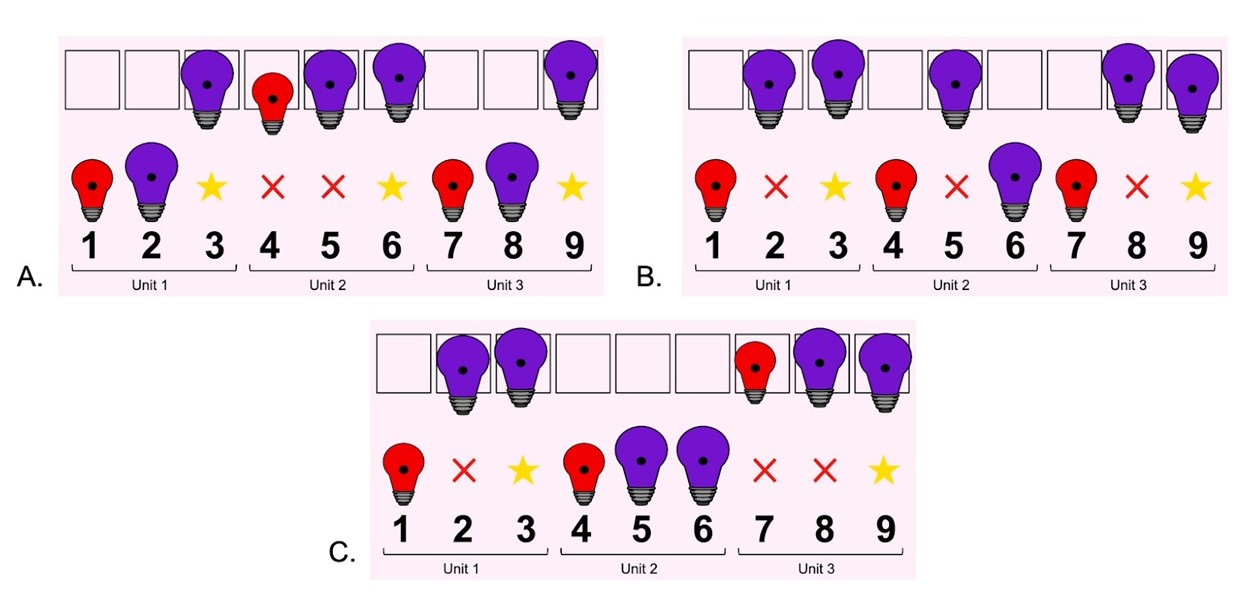
\includegraphics[width=\textwidth]{future/figures/pattern_strat.jpg}
  \caption[Examples of the pattern-relevant strategies.]{Examples of the pattern-relevant strategies observed in the pattern transfer task: A) Unconstrained chunking - searching under at least one shape from all three repeated units, B) Shape matching - searching only under the large shapes, and C) Constrained chunking - searching under shapes from only two of the three repeated units.
}
  \label{fig:pattern-strat}
\end{figure}

Though there were no significant differences in performance on the pattern abstraction task, children interestingly used different strategies. One researcher and a research assistant coded children's patterning strategies blind to condition according to three main categories: pattern-irrelevant, pattern-relevant, and advanced pattern strategies. Disagreements and sub-strategies were discussed and resolved between the two raters. A sequential strategy (choosing shapes from either left to right or right to left in a sequential order) and spatial grouping (searching only in closely proximal shapes) represented the two sub-strategies in the pattern-irrelevant strategies as they do not demonstrate an understanding of the underlying pattern. Unconstrained chunking (searching at least one shape in each of the three repeating units)(Figure \ref{fig:pattern-strat}A), shape matching (searching only in the B shapes in each ABB unit)(Figure \ref{fig:pattern-strat}B), and constrained chunking (searching at least one shape in only two of the three repeating units)(Figure \ref{fig:pattern-strat}C) represented the three pattern-relevant strategies as they demonstrate some understanding of the underlying pattern. Exploit (finding all three stars in a row) represented the most advanced strategy as it demonstrates a clear understanding of not only the underlying pattern, but also the understanding of where each star is within the pattern. Table \ref{table:pattern_strats} shows the various patterning strategies and the frequency of participants who engaged in each strategy. 

\begin{table}[]
\centering
\caption{Children engaged in various strategies to solve the pattern transfer task. In both
the \textit{exploration} and \textit{demonstration} conditions, six-year-olds engaged in more mature, pattern-relevant
strategies than five-year-olds.}
\label{table:pattern_strats}
\begin{tabular}{rrcccc}
\hline
\multicolumn{1}{c}{Strategy Type} & \multicolumn{1}{c}{Sub-Strategies} & \multicolumn{2}{c}{5-year-olds} & \multicolumn{2}{c}{6-year-olds} \\
\multicolumn{1}{l}{} &  & \multicolumn{1}{l}{Explore} & \multicolumn{1}{l}{Demonstrate} & \multicolumn{1}{l}{Explore} & \multicolumn{1}{l}{Demonstrate} \\ \hline
Pattern-Irrelevant & Sequential & 1 & 5 & 2 & 1 \\
 & \begin{tabular}[c]{@{}r@{}}Spatial \\ Grouping\end{tabular} & 3 & 2 & 0 & 1 \\ \hline
Pattern-Relevant & \begin{tabular}[c]{@{}r@{}}Unconstrained\\ Chunking\end{tabular} & 7 & 5 & 7 & 8 \\
 & \begin{tabular}[c]{@{}r@{}}Constrained\\ Chunking\end{tabular} & 1 & 1 & 0 & 1 \\
 & \begin{tabular}[c]{@{}r@{}}Shape\\ Matching\end{tabular} & 2 & 2 & 1 & 2 \\ \hline
Advanced & Exploit & 3 & 2 & 7 & 4 \\ \hline
\end{tabular}
\end{table}

For five-year-olds in both conditions, a majority of children used pattern-relevant strategies in the pattern transfer task (10 out of 17 for the \textit{exploration} condition and 9 out of 17 for the \textit{demonstration} condition). A majority of six-year-old \textit{demonstration} condition participants also used pattern-relevant strategies (11 out of 17). 7 of the 17 six-year-old \textit{exploration} condition participants used the most adavanced exploit strategy, finding all three stars consecutively, compared to 4 of the 17 six-year-old \textit{demonstration} condition participants. These preliminary results suggest that exploration may influence implicit pattern recognition and lead to better transfer and abstraction of patterns in new contexts.

\subsection{Discussion}
We provide preliminary evidence of the efficacy of utilizing exploration as a learning strategy in patterning for young children. This section discusses how exploration can further impact pedagogical methods and learning outcomes for children.

\subsubsection{Exploration Encourages Active Engagement}
Our results demonstrate that children can implicitly learn patterns even without direct instruction or feedback. As opposed to the \textit{demonstration} condition, exploration enabled children to make sense of the pattern on their own. This active engagement may be a reason why we observed a trend of more \textit{exploration} condition children engaging in an advanced, exploit strategy in the pattern transfer task. Because they were able to engage with the pattern previously, they may have been better able to connect the two structurally similar patterns. 

Some children spontaneously explained their pattern reasoning during the pattern transfer task. For example, one five-year-old \textit{exploration} participant said during the pattern transfer task, ``\textit{It looks like a pattern right? Listen, it’s star, x, x, star, x, x, star, x, x.}'' Similarly, a six-year-old in the \textit{demonstration} condition referred to the pattern from right to left and explained, ``\textit{This is the pattern. It’s no star, no star, star, no star, no star, star, no star, no star, star}.'' Other children also pointed out the star and x pattern, but did so with respect to the shapes. For example, a five-year-old in the \textit{exploration} condition stated, ``\textit{After two houses, one house has a star inside of it}.'' A 6-year-old in the \textit{exploration} condition similarly expressed, “\textit{Wait, I realized something. There’s a pattern: two houses that don’t have a star and then one house that does have a star}.” Both children successfully found all the hidden stars using the advanced exploit strategy. Though not explicitly told the pattern to finding the hidden stars, both five- and six-year-old children demonstrated knowledge of the underlying pattern. More specifically, they showed understanding of the repeating pattern unit. Future interventions that utilize active engagement through exploration show promise for developing a general ability to identify repeating units within a pattern even without direct instruction.

Our study examined the immediate learning effects of exploration. Future work could examine the longitudinal effects of using exploration as a learning strategy. For example, inventive activities that ask learners to produce original solutions prior to direct instruction prepare learners for future learning because they can connect their preconceptions to new knowledge gained \cite{Schwartz2004}. Exploratory learning strategies may have a similar impact, priming children to pay attention to the high-level pattern structure rather than the specific components (\textit{i.e.} shapes or stimuli) of the pattern. 

\subsubsection{Exploration Needs to Be Goal-Directed}
Exploration as a problem-solving strategy can be inefficient, particularly when the goal itself may be ambiguous \cite{fraser2019replay,kirschner2006,tuovinen1999comparison}. In our task, children had a clear goal to accomplish: find the hidden stars using a pattern. With this goal, children were directed in their exploratory efforts, which emerged through the strategies we observed. In addition, the task included immediate feedback. Children could see whether the house they selected contained a star underneath right after selection. This feedback may have helped children test and update their hypotheses of the pattern \cite{sumner2019,wilson2021}. While the pattern for finding the hidden stars was concrete, the differing strategies children used suggest that goal-directed exploration and immediate feedback may highlight alternative paths to solving the pattern. 28 of the 34 children in the \textit{exploration} condition and 23 of the 34 children in the \textit{demonstration} condition used some form of pattern-relevant strategy, demonstrating some understanding of the underlying pattern unit. In other forms of creative problem-solving, exploratory strategies should similarly enable people to quickly receive feedback and provide a clear goal to achieve through exploration.

\subsubsection{Summary}
We investigated whether exploration could help children learn and transfer patterns. In a between-subjects experiment, children either explored patterns themselves or watched a demonstration of the pattern. Our results suggest a trend that exploration may encourage more active engagement and highlight underlying structure. Future interventions that utilize exploration as a problem-solving strategy should provide mechanisms for immediate feedback and goal direction.

\subsubsection{Acknowledgements}
We thank our participants and their families for the time and participation in this task. We also thank Amberley Stein for assisting with coding patterning strategies.

This chapter, in part, is currently being prepared for submission for publication of the material by Tricia J. Ngoon, Vivian Leung, and Caren M. Walker. The dissertation author was the primary investigator and author of this material.
